\XtoCBlock{AutoSwitch}
\label{block:AutoSwitch}
\begin{figure}[H]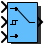
\includegraphics{AutoSwitch}\end{figure} 

\begin{XtoCtabular}{Inports}
In1 & Input \#1\tabularnewline
\hline
Switch & Input \#2: Threshold signal\tabularnewline
\hline
In3 & Input \#3\tabularnewline
\hline
\end{XtoCtabular}


\begin{XtoCtabular}{Outports}
Out & Either value of input \#1 or input \#3 dependent on value of input \#2\tabularnewline
\hline
\end{XtoCtabular}

\begin{XtoCMaskParamTabular}{Mask Parameters}
\rowcolor[gray]{0.8}\textbf{Name} & \textbf{ID} & \textbf{Description}\tabularnewline\hline
Thresh\_up & 1 & Threshold level for rising switch signal\tabularnewline
\hline
Thresh\_down & 2 & Threshold level for falling switch signal\tabularnewline
\hline
\end{XtoCMaskParamTabular}

\subsubsection*{Description:}
Switch between In1 and In3 dependent on Switch signal:

    Switch signal rising:  Switch >= Threshold up --> Out = In1

    Switch signal falling: Switch <  Threshold down --> Out = In3

% include optional documentation file
\InputIfFileExists{\XcHomePath/Library/General/Doc/AutoSwitch_Info.tex}{\vspace{1ex}}{}

\subsubsection*{Implementations:}
\begin{tabular}{l l}
\textbf{FiP16} & 16 Bit Fixed Point Implementation\tabularnewline
\textbf{FiP32} & 32 Bit Fixed Point Implementation\tabularnewline
\textbf{Float32} & 32 Bit Floating Point Implementation\tabularnewline
\textbf{Float64} & 64 Bit Floating Point Implementation\tabularnewline
\end{tabular}

\XtoCImplementation{FiP16}
\nopagebreak[0]

16 Bit Fixed Point Implementation

\begin{XtoCtabular}{Inports Data Type}
In1 & int16\tabularnewline
\hline
Switch & int16\tabularnewline
\hline
In3 & int16\tabularnewline
\hline
\end{XtoCtabular}

\begin{XtoCtabular}{Outports Data Type}
Out & int16\tabularnewline
\hline
\end{XtoCtabular}

\ifdefined \AddTestReports
\InputIfFileExists{\XcHomePath/Library/General/Doc/Test-Results/Test_AutoSwitch_FiP16.tex}{}{}
\fi
\XtoCImplementation{FiP32}
\nopagebreak[0]

32 Bit Fixed Point Implementation

\begin{XtoCtabular}{Inports Data Type}
In1 & int32\tabularnewline
\hline
Switch & int32\tabularnewline
\hline
In3 & int32\tabularnewline
\hline
\end{XtoCtabular}

\begin{XtoCtabular}{Outports Data Type}
Out & int32\tabularnewline
\hline
\end{XtoCtabular}

\ifdefined \AddTestReports
\InputIfFileExists{\XcHomePath/Library/General/Doc/Test-Results/Test_AutoSwitch_FiP32.tex}{}{}
\fi
\XtoCImplementation{Float32}
\nopagebreak[0]

32 Bit Floating Point Implementation

\begin{XtoCtabular}{Inports Data Type}
In1 & float32\tabularnewline
\hline
Switch & float32\tabularnewline
\hline
In3 & float32\tabularnewline
\hline
\end{XtoCtabular}

\begin{XtoCtabular}{Outports Data Type}
Out & float32\tabularnewline
\hline
\end{XtoCtabular}

\ifdefined \AddTestReports
\InputIfFileExists{\XcHomePath/Library/General/Doc/Test-Results/Test_AutoSwitch_Float32.tex}{}{}
\fi
\XtoCImplementation{Float64}
\nopagebreak[0]

64 Bit Floating Point Implementation

\begin{XtoCtabular}{Inports Data Type}
In1 & float64\tabularnewline
\hline
Switch & float64\tabularnewline
\hline
In3 & float64\tabularnewline
\hline
\end{XtoCtabular}

\begin{XtoCtabular}{Outports Data Type}
Out & float64\tabularnewline
\hline
\end{XtoCtabular}

\ifdefined \AddTestReports
\InputIfFileExists{\XcHomePath/Library/General/Doc/Test-Results/Test_AutoSwitch_Float64.tex}{}{}
\fi
